\section{Informationstheorie, Algorithmen und Datenqualität}

% ─────────────────────────────────────────────────────────────────────────────
\subsection{Teile-und-Herrsche-Prinzip sowie Prinzip des dynamischen Programmierens}

\definition{\textbf{Teile und Herrsche} (Divide and Conquer): Umfangreiche Aufgaben werden in kleinere Teilprobleme zerlegt, diese werden gelöst, und die Teillösungen zur Gesamtlösung zusammengesetzt. Realisierung meistens mittels Rekursion.
    \begin{enumerate}[leftmargin=2em]
        \item \textbf{Teile:} Problem in kleinere Teilprobleme zerlegen.
        \item \textbf{Herrsche:} Jedes Teilproblem (rekursiv) lösen.
        \item \textbf{Verbinde:} Teillösungen zur Gesamtlösung zusammensetzen.
    \end{enumerate}}

\textbf{Beispiel Mergesort:}
\begin{itemize}[leftmargin=1.5em]
    \item \textbf{Teile:} Datensatz in zwei Hälften aufteilen.
    \item \textbf{Herrsche:} Jede Hälfte getrennt (rekursiv) sortieren -- bis jeder Teildatensatz nur noch aus einem Element besteht.
    \item \textbf{Verbinde:} Zwei sortierte Hälften ordnungserhaltend zusammenführen (merge). Laufzeit: $\mathcal{O}(n \log n)$.
\end{itemize}

\begin{figure}[H]
    \centering
    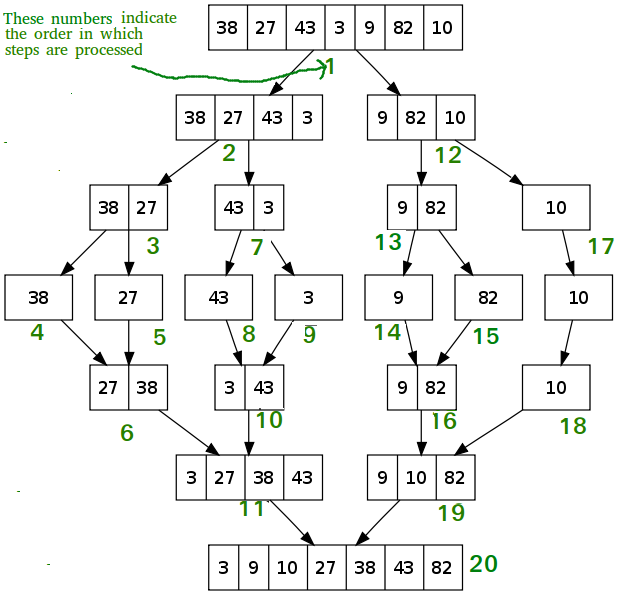
\includegraphics[width=0.45\textwidth]{assets/mergesort.png}
\end{figure}

\beispiel{\textbf{Mergesort konkret:} Gegeben sei die Liste $[5, 2, 8, 1, 9, 3]$.
\begin{enumerate}[leftmargin=2em]
    \item \textbf{Teile:} $[5, 2, 8]$ und $[1, 9, 3]$, dann weiter: $[5]$, $[2, 8]$, $[1]$, $[9, 3]$ usw.
    \item \textbf{Herrsche:} Einzel-Elemente sind trivial sortiert.
    \item \textbf{Verbinde:} $[2, 8]$ aus $[2]$ und $[8]$; $[2, 5, 8]$ aus $[5]$ und $[2, 8]$; analog $[1, 3, 9]$; schließlich $[1, 2, 3, 5, 8, 9]$.
\end{enumerate}
Zu jedem Zeitpunkt werden nur zwei sortierte Teilarrays verglichen -- daher $\mathcal{O}(n \log n)$ auch im schlechtesten Fall.}

\textbf{Quicksort} funktioniert ähnlich, trennt aber anhand eines Pivot-Elements: Alle Elemente kleiner als das Pivot kommen links, alle größeren rechts. Im schlechtesten Fall (bereits sortierte Liste, schlechtes Pivot) $\mathcal{O}(n^2)$, im Durchschnitt $\mathcal{O}(n \log n)$. In der Praxis oft schneller als Mergesort, da kein Hilfsarray benötigt wird (in-place).

\definition{\textbf{Dynamisches Programmieren:} Rekursiv formulierte Aufgaben sind oft nicht am besten rekursiv lösbar, weil dieselben Teilprobleme exponentiell oft neu berechnet werden.

    \textbf{Idee:} Am einfachsten Punkt ansetzen, schrittweise vorarbeiten und \textbf{Zwischenergebnisse speichern} (Memoization / Tabellierung), um wiederholte Berechnung zu vermeiden.

    \textbf{Zwei Varianten:}
    \begin{itemize}[leftmargin=1.5em]
        \item \textbf{Top-Down mit Memoization:} Rekursiver Aufruf wie gewohnt, aber Ergebnisse werden in einer Tabelle gespeichert und bei erneutem Bedarf nachgeschlagen.
        \item \textbf{Bottom-Up (Tabellierung):} Iterativer Aufbau der Lösungstabelle vom kleinsten Teilproblem aufwärts -- kein Rekursions-Overhead.
    \end{itemize}}

\beispiel{\textbf{Fibonacci-Folge} $f_n = f_{n-1} + f_{n-2}$, $f_1 = f_2 = 1$:
\begin{itemize}[leftmargin=1.5em]
    \item \textbf{Naiv rekursiv:} $f_5$ ruft $f_4$ und $f_3$ auf; $f_4$ ruft erneut $f_3$ und $f_2$ auf -- $f_3$ wird mehrfach berechnet. Gesamtzahl der Aufrufe wächst exponentiell: $\mathcal{O}(2^n)$.
    \item \textbf{Dynamisch:} Berechne $f_1=1, f_2=1, f_3=2, f_4=3, f_5=5, \ldots$ der Reihe nach und speichere jeden Wert. Jedes $f_k$ wird genau einmal berechnet: $\mathcal{O}(n)$.
\end{itemize}}

\textbf{Weiteres klassisches Beispiel -- Rucksackproblem (0/1 Knapsack):} Gegeben $n$ Gegenstände mit Gewicht $w_i$ und Wert $v_i$ sowie maximale Traglast $W$. Die Rekurrenz lautet:
\formel{dp[i][c] = \max\bigl(dp[i-1][c],\; v_i + dp[i-1][c-w_i]\bigr)}
d.\,h.\ entweder man nimmt Gegenstand $i$ nicht (Wert bleibt $dp[i-1][c]$) oder man nimmt ihn (Wert erhöht sich um $v_i$, Kapazität sinkt um $w_i$). Laufzeit: $\mathcal{O}(nW)$.

\textbf{Bellman-Gleichung:} Das dynamische Programmieren liegt der Bellman-Gleichung zugrunde, die zentral im \textbf{Reinforcement Learning} ist:
\formel{V^*(s) = \max_a \Bigl[R(s,a) + \gamma \sum_{s'} P(s'|s,a)\, V^*(s')\Bigr]}
Der optimale Wert eines Zustands $s$ ergibt sich als Funktion der optimalen Werte der Folgezustände $s'$ -- typisches Bottom-up-Vorgehen.

\textbf{Abgrenzung:} Teile-und-Herrsche zerlegt das Problem in \emph{unabhängige} Teilprobleme (kein Überlapp). Dynamisches Programmieren ist geeignet, wenn Teilprobleme \emph{überlappen} -- dieselben Teilprobleme mehrfach auftreten und deren Ergebnisse wiederverwendet werden können.

\begin{figure}[H]
    \centering
    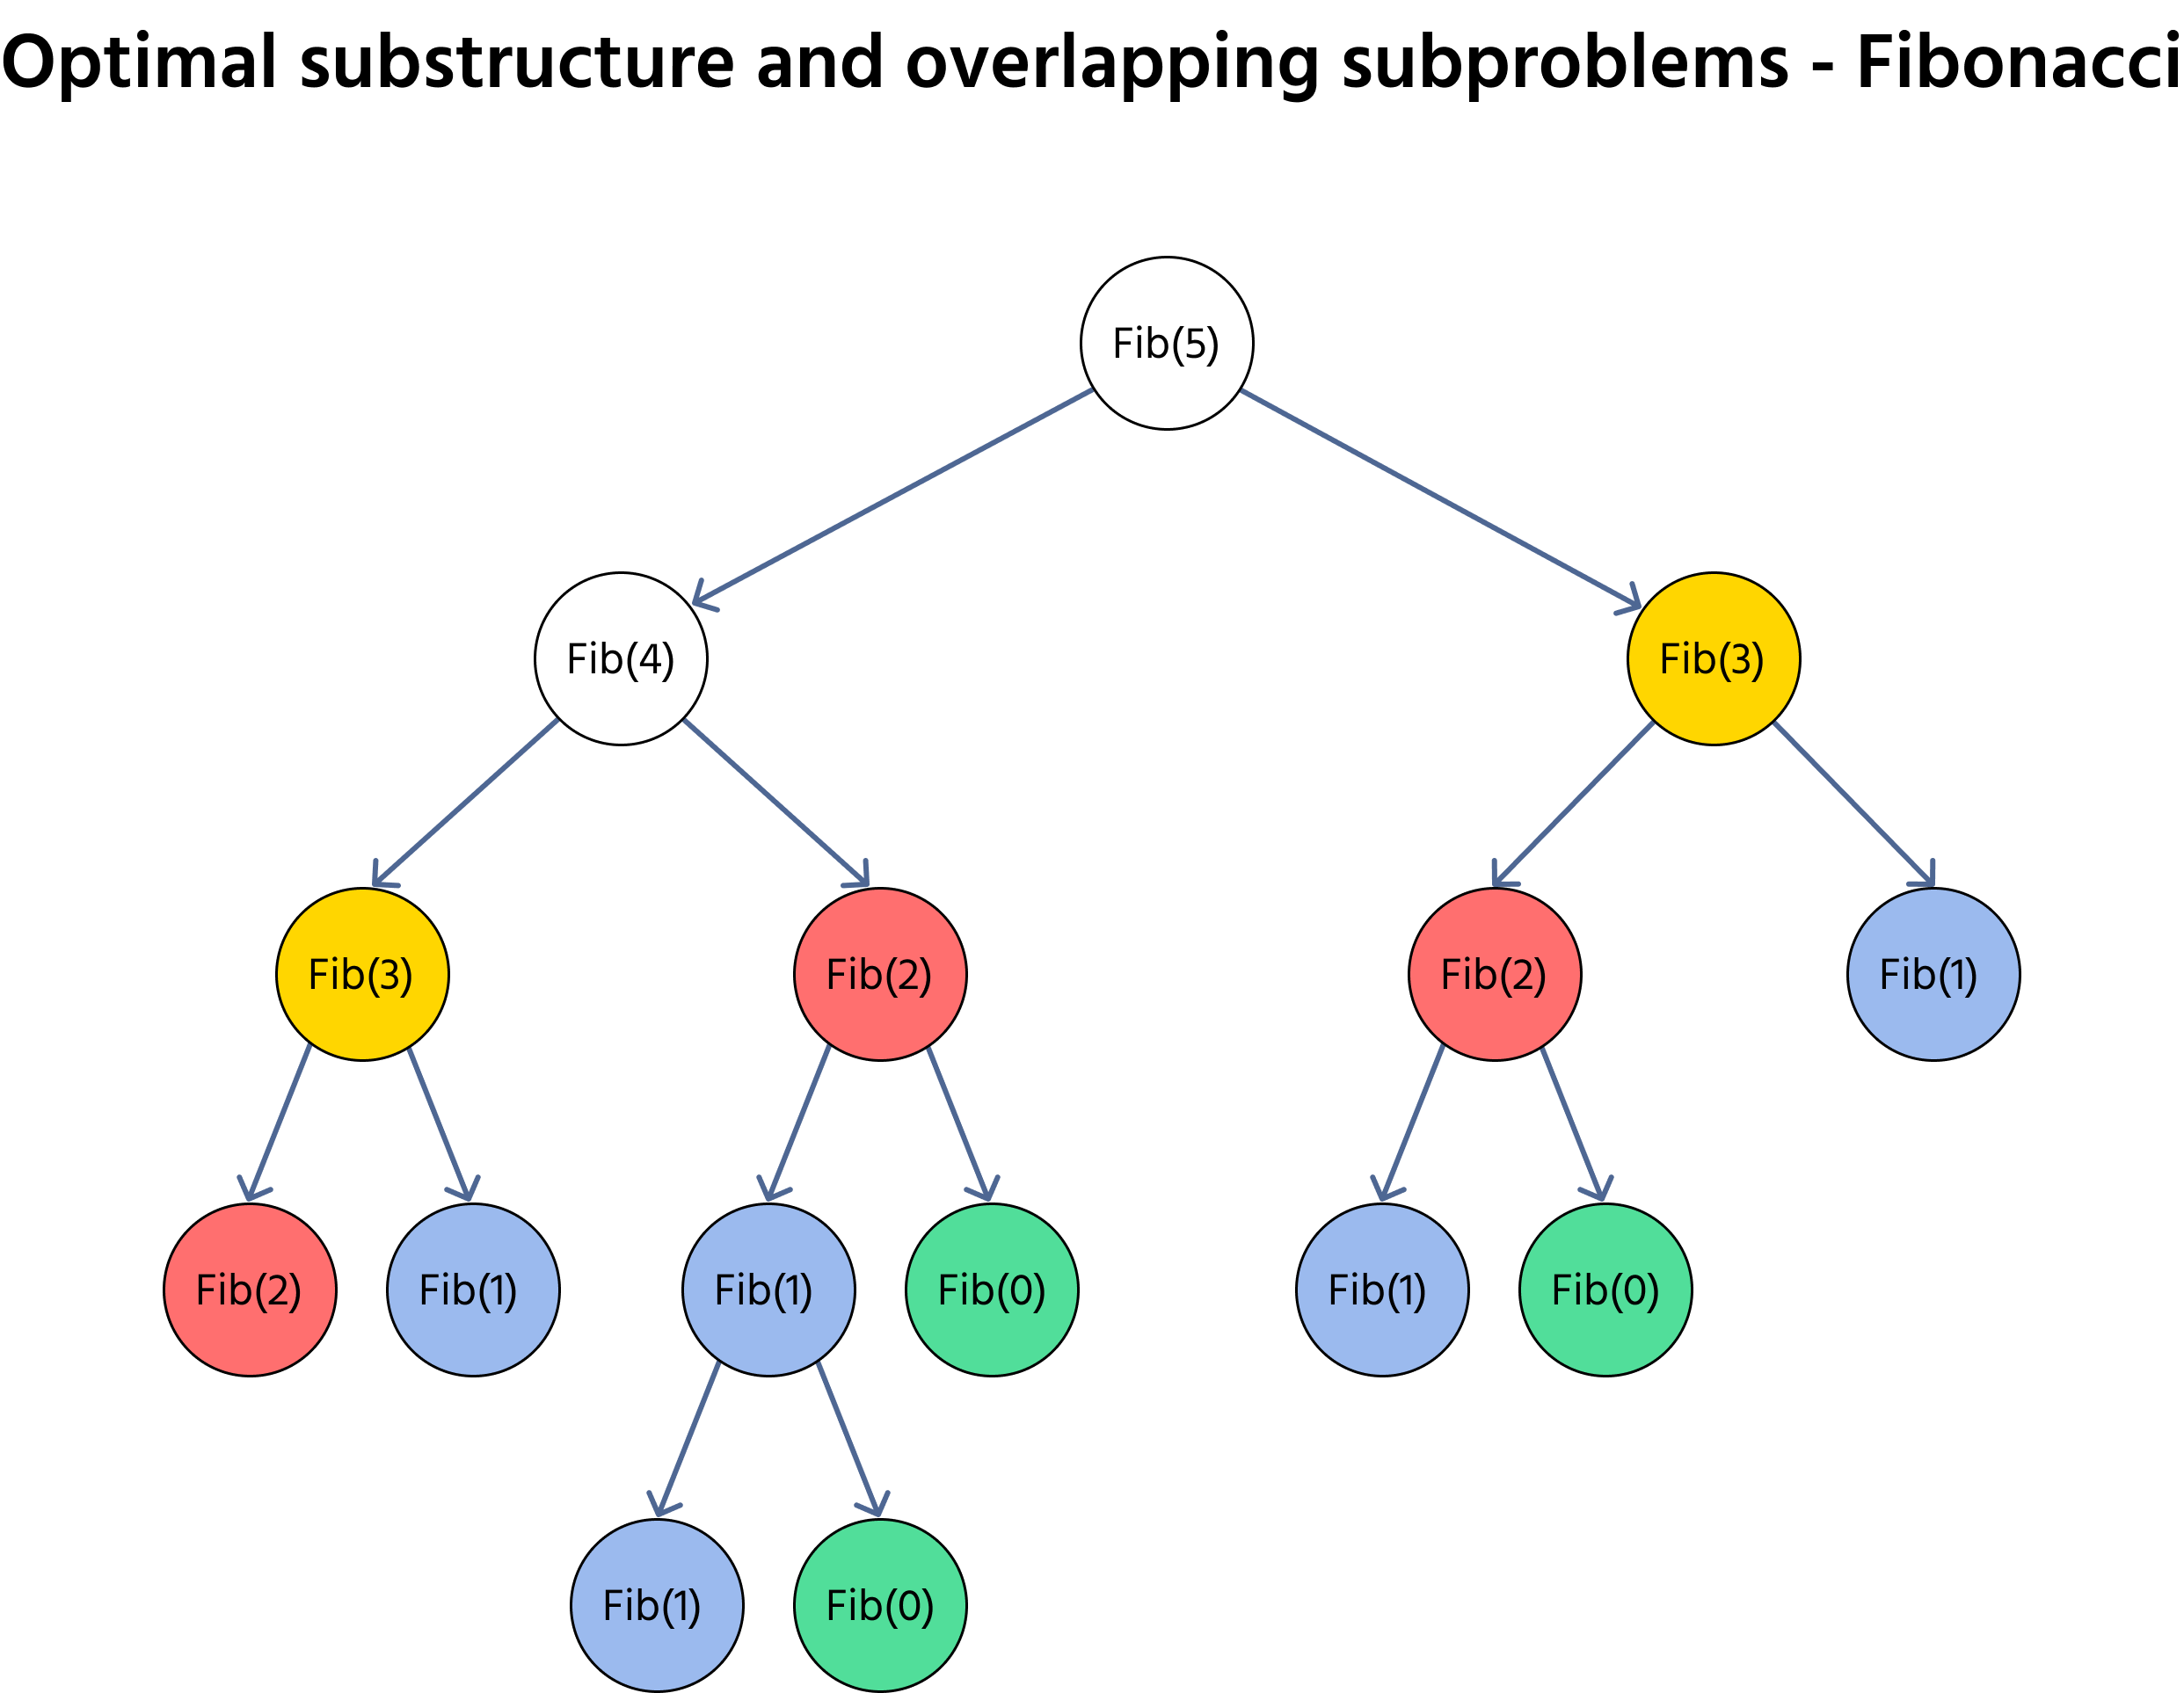
\includegraphics[width=0.45\textwidth]{assets/dyn_prog.png}
\end{figure}

\newpage
% ─────────────────────────────────────────────────────────────────────────────

\subsection{Informationsentropie: Definition, Bedeutung, Einsatzmöglichkeiten}

\textbf{Informationsgehalt:} Für ein Ereignis mit Wahrscheinlichkeit $p_i$ ist der Informationsgehalt:
\formel{I(p_i) = \log_2\frac{1}{p_i} = -\log_2 p_i \quad \text{(in Bit)}}
Seltene Ereignisse tragen mehr Information: Ein Münzwurf (50\,\%) liefert $I = 1$\,Bit; ein Würfelergebnis (1/6) liefert $I = \log_2 6 \approx 2{,}58$\,Bit. Für $n$ gleichwahrscheinliche Ereignisse: $I = \log_2 n$.

\definition{\textbf{Informationsentropie} $H$ ist der \emph{Erwartungswert} des Informationsgehalts einer Verteilung $\bm{p} = (p_1,\ldots,p_N)$:
    \formel{H(\bm{p}) = -K\sum_{i=1}^{N} p_i \lg p_i}
    mit Konstante $K > 0$ und Logarithmus $\lg$. Wahl von $K$ und $\lg$ legen die Einheit fest: $K=1$, $\lg = \log_2$ $\Rightarrow$ Bit; $K=1$, $\lg = \ln$ $\Rightarrow$ Nat. Für $p_i = 0$ setzt man den Summanden $= 0$ (da $\lim_{p\to 0} p\log p = 0$). Im diskreten Fall gilt stets $H \geq 0$.}

\textbf{Eigenschaften:}
\begin{itemize}[leftmargin=1.5em]
    \item $H$ ist \textbf{maximal} für Gleichverteilung: $p_i = \frac{1}{N}$ für alle $i$ $\Rightarrow$ $H_{\max} = \log_2 N$ Bit. Maximale Unsicherheit entspricht maximaler Information pro Symbol.
    \item $H = 0$ wenn ein Ereignis sicher eintritt ($p_i = 1$ für ein $i$): keine Unsicherheit, kein Informationsgewinn durch Beobachtung.
    \item \textbf{Konkavität:} $H$ ist eine konkave Funktion der Wahrscheinlichkeiten -- jede Annäherung an die Gleichverteilung erhöht $H$.
    \item Für eine \textbf{kontinuierliche} Verteilung $p(x)$: $H[p] = -K\int_a^b p(x)\lg p(x)\,\mathrm{d}x$ (differentielle Entropie); kann negativ werden, da $p(x) > 1$ möglich ist.
\end{itemize}

\beispiel{\textbf{Vier Symbole mit ungleicher Verteilung:} $p_A=\frac{1}{2}$, $p_B=\frac{1}{4}$, $p_C=p_D=\frac{1}{8}$.
\[
H = -\tfrac{1}{2}\log_2\tfrac{1}{2} - \tfrac{1}{4}\log_2\tfrac{1}{4} - \tfrac{1}{8}\log_2\tfrac{1}{8} - \tfrac{1}{8}\log_2\tfrac{1}{8}
  = \tfrac{1}{2}{\cdot}1 + \tfrac{1}{4}{\cdot}2 + \tfrac{1}{8}{\cdot}3 + \tfrac{1}{8}{\cdot}3 = 1{,}75 \text{ Bit/Symbol.}
\]
Zum Vergleich: Bei Gleichverteilung ($p_i = \frac{1}{4}$) wäre $H_{\max} = \log_2 4 = 2$\,Bit/Symbol -- die ungleiche Verteilung reduziert die Entropie, weil $A$ sehr vorhersehbar ist.

\textbf{Optimale Codierung (Huffman):} $A \hat{=} 0$ (1 Bit), $B \hat{=} 10$ (2 Bit), $C \hat{=} 110$ (3 Bit), $D \hat{=} 111$ (3 Bit). Mittlere Codewortlänge: $\frac{1}{2}{\cdot}1 + \frac{1}{4}{\cdot}2 + \frac{1}{8}{\cdot}3 + \frac{1}{8}{\cdot}3 = 1{,}75$\,Bit/Symbol $= H$ -- der Huffman-Code erreicht hier die Entropie-Untergrenze exakt.}

\textbf{Einsatzmöglichkeiten:}
\begin{itemize}[leftmargin=1.5em]
    \item \textbf{Datenkompression:} Shannons Quellencodierungstheorem besagt, dass die mittlere Codewortlänge einer verlustfreien Codierung mindestens $H$ Bit/Symbol betragen muss. Huffman-Codes erreichen diese Grenze für ganzzahlige Codewortlängen; arithmetische Codes kommen ihr beliebig nah.
    \item \textbf{Kanalkapazität:} Die Kapazität $C$ eines Kanals gibt an, wie viele Bits pro Symbol fehlerfrei übertragen werden können. Entropie quantifiziert den Informationsfluss und damit den Auslastungsgrad des Kanals.
    \item \textbf{Entscheidungsbäume (Machine Learning):} Der \emph{Information Gain} eines Features $X$ bezüglich Zielvariable $Y$ ist $IG(Y, X) = H(Y) - H(Y|X)$. Ein gutes Split-Kriterium wählt das Feature mit maximalem Information Gain.
    \item \textbf{Kreuzentropie als Verlustfunktion:} Direkte Anwendung in neuronalen Netzen für Klassifikationsaufgaben (siehe nächster Abschnitt).
\end{itemize}

\newpage
% ─────────────────────────────────────────────────────────────────────────────

\subsection{Kreuzentropie und KL-Divergenz}

Betrachte zwei Wahrscheinlichkeitsverteilungen $p$ (wahre/empirische Verteilung) und $q$ (Modellverteilung) auf einem Ereignisraum $X$.

\definition{\textbf{Kreuzentropie (Cross-Entropy):}
    \formel{H_\mathrm{cross}(p \| q) = -\sum_{x \in X} p(x)\lg q(x)}
    Interpretation: durchschnittliche Anzahl der Bits, um ein Symbol zu beschreiben, wenn die Codierung für Modellverteilung $q$ statt für die wahre Verteilung $p$ optimiert ist. Es gilt stets $H_\mathrm{cross}(p\|q) \geq H(p)$, mit Gleichheit genau dann, wenn $q = p$.}

\definition{\textbf{Kullback-Leibler-Divergenz (KL-Divergenz, relative Entropie):}
    \formel{D_\mathrm{KL}(p\|q) = \sum_{x \in X} p(x)\lg\frac{p(x)}{q(x)} = H_\mathrm{cross}(p\|q) - H(p)}
    Interpretation: durchschnittliche Anzahl der \emph{zusätzlichen} Bits gegenüber dem theoretischen Minimum, die entstehen, weil $q$ statt $p$ zur Codierung verwendet wird.

    \textbf{Eigenschaften:}
    \begin{itemize}[leftmargin=1.5em]
        \item $D_\mathrm{KL}(p\|q) \geq 0$ (Gibbs'sche Ungleichung), mit Gleichheit genau dann wenn $p = q$.
        \item \textbf{Nicht symmetrisch:} I.\,A.\ $D_\mathrm{KL}(p\|q) \neq D_\mathrm{KL}(q\|p)$ -- daher kein echter Abstand im metrischen Sinne.
        \item \textbf{Forward vs.\ Reverse KL:} $D_\mathrm{KL}(p\|q)$ (Forward) bestraft Regionen, in denen $q(x) \ll p(x)$ -- das Modell unterschätzt die wahre Dichte. $D_\mathrm{KL}(q\|p)$ (Reverse) bestraft Regionen, in denen $p(x) \ll q(x)$.
    \end{itemize}}

\beispiel{\textbf{Zwei Münzen:} Sei $p = (0{,}9,\, 0{,}1)$ (stark verzerrte Münze) und $q = (0{,}5,\, 0{,}5)$ (faire Münze).
\[
H(p) = -0{,}9\log_2 0{,}9 - 0{,}1\log_2 0{,}1 \approx 0{,}469 \text{ Bit}
\]
\[
H_\mathrm{cross}(p\|q) = -0{,}9\log_2 0{,}5 - 0{,}1\log_2 0{,}5 = 1{,}0 \text{ Bit}
\]
\[
D_\mathrm{KL}(p\|q) = 1{,}0 - 0{,}469 = 0{,}531 \text{ Bit}
\]
Kodiert man Symbole aus $p$ mit dem für $q$ optimierten Code, braucht man im Mittel 0{,}531 Bit mehr pro Symbol -- das ist die ``Strafe'' für das falsche Modell.}

\textbf{Einsatz in Machine Learning -- Klassifikation:} Bei One-hot-Encoding $\bm{y} = (y_1,\ldots,y_n)$ und Modellausgabe $\hat{\bm{y}} = (\hat{y}_1,\ldots,\hat{y}_n)$ mit Softmax ($\hat{y}_i \geq 0$, $\sum \hat{y}_i = 1$):

\begin{itemize}[leftmargin=1.5em]
    \item \textbf{Least-Squares-Loss:} $L_\mathrm{LSq} = \sum_i (\hat{y}_i - y_i)^2$ -- bei falsch klassifizierten Beispielen mit hoher Konfidenz ($\hat{y}_i \approx 0$) ist der Gradient sehr klein (Sättigungsproblem).
    \item \textbf{Kreuzentropie-Loss:} $L_\mathrm{CE} = -\sum_i y_i \ln \hat{y}_i$ -- für One-hot-Label vereinfacht sich dies zu $L_\mathrm{CE} = -\ln \hat{y}_c$, wobei $c$ die wahre Klasse ist. Dieser Wert divergiert für $\hat{y}_c \to 0$, was falsch klassifizierten Beispielen einen großen Gradienten gibt -- kein Sättigungsproblem.
\end{itemize}

\beispiel{Für $\bm{y} = (1,0,0)$ und $\hat{\bm{y}} = (0{,}1,\, 0{,}7,\, 0{,}2)$ (stark falsch klassifiziert) $L_\mathrm{CE} = -\ln 0{,}1 \approx 2{,}30$. Für $\hat{\bm{y}} = (0{,}9,\, 0{,}05,\, 0{,}05)$ (korrekt klassifiziert): $L_\mathrm{CE} = -\ln 0{,}9 \approx 0{,}105$. Die Kreuzentropie bestraft falsche Klassifikationen mit hoher Konfidenz stark -- was zu schnellerer Konvergenz führt.}

\textbf{Zusammenhang:} Da $H(p)$ konstant bzgl.\ $q$, ist Minimierung von $H_\mathrm{cross}(p\|q)$ äquivalent zur Minimierung von $D_\mathrm{KL}(p\|q)$ -- das Training eines Klassifikators entspricht damit einer KL-Minimierung zwischen empirischer und Modellverteilung.

\newpage
% ─────────────────────────────────────────────────────────────────────────────

\subsection{Fehlererkennende und -korrigierende Codes}

\textbf{Motivation:} Bei jeder Datenübertragung (WLAN, Glasfaser, DVD-Lesen, manuelle Eingabe) können Fehler auftreten. Mit systematischen Codes lassen sich typische Fehler erkennen oder sogar korrigieren, ohne die gesamte Übertragung zu wiederholen.

\textbf{Fehlertypen:} Die häufigsten sind \emph{Einzelbitfehler} bei Zeichenübertragung und \emph{Ziffernfehler} (falsche Ziffer oder Vertauschung benachbarter Ziffern) bei numerischen Codes. Zusätzlich treten \emph{Büschelfehler} (Burst Errors) auf -- zusammenhängende Fehlerfolgen, z.\,B.\ durch Kratzer auf einer CD.

\definition{\textbf{Hamming-Distanz:} Die Hamming-Distanz $d(c_1, c_2)$ zweier Codewörter $c_1, c_2$ ist die Anzahl der Positionen, an denen sie sich unterscheiden. Ein Code mit minimaler Hamming-Distanz $d_{\min}$ kann:
    \begin{itemize}[leftmargin=1.5em]
        \item bis zu $d_{\min} - 1$ Fehler \textbf{erkennen},
        \item bis zu $\lfloor\frac{d_{\min}-1}{2}\rfloor$ Fehler \textbf{korrigieren}.
    \end{itemize}}

\definition{\textbf{Paritätsbit (ASCII):} Der 7-Bit ASCII-Code nutzt das 8.\ Bit als Prüfbit. Das Paritätsbit wird so gesetzt, dass die Gesamtzahl der 1-Bits gerade ist. Findet sich bei Empfang ein Byte mit ungerader Anzahl an 1-Bits, liegt ein Fehler vor. $d_{\min} = 2$: erkennt Einzelfehler, kann aber nicht korrigieren und übersieht Doppelfehler.}

\definition{\textbf{ISBN-10-Code:} Jede Ziffer $z_i$ wird mit ihrer Position multipliziert, die Summe wird modulo 11 reduziert:
\formel{\text{Prüfziffer} = \left(\sum_{i=1}^{9} i \cdot z_i\right) \bmod 11}
Da $\mathbb{Z}_{11}$ ein Körper ist (also nullteilerfrei), werden \emph{beliebige Einzelziffernfehler} und alle \emph{Vertauschungen benachbarter Ziffern} erkannt. Bei Prüfziffer $= 10$ wird das Symbol \glqq X\grqq{} verwendet.}

\beispiel{\textbf{ISBN-10 Prüfung:} Sei die ISBN \texttt{0-306-40615-?}. Berechnung:
\[
\sum_{i=1}^{9} i \cdot z_i = 1{\cdot}0 + 2{\cdot}3 + 3{\cdot}0 + 4{\cdot}6 + 5{\cdot}4 + 6{\cdot}0 + 7{\cdot}6 + 8{\cdot}1 + 9{\cdot}5 = 0+6+0+24+20+0+42+8+45 = 145
\]
$145 \bmod 11 = 2$ (da $11 \cdot 13 = 143$) $\Rightarrow$ Prüfziffer ist \textbf{2}.}

\textbf{Fehlerkorrigierende Codes:}
\begin{itemize}[leftmargin=1.5em]
    \item \textbf{Hamming-Code (7,4):} Kodiert 4 Datenbits in 7 Bits durch Hinzufügen von 3 Paritätsbits an Positionen $2^0=1$, $2^1=2$, $2^2=4$. Jedes Paritätsbit überwacht eine andere Teilmenge der Datenbits. Das Fehlersyndrom (Muster der nicht-stimmigen Paritätsbits) zeigt die binäre Position des Fehlers an. $d_{\min} = 3$: korrigiert alle Einzelfehler. Mit einem zusätzlichen Gesamtparitätsbit ($d_{\min} = 4$): korrigiert Einzelfehler \emph{und} erkennt Doppelfehler.

    \item \textbf{Reed-Solomon-Code:} Kodiert Daten als Koeffizienten eines Polynoms $p(x)$ vom Grad $k-1$ und überträgt $n > k$ Auswertungen an fest gewählten Stützstellen. Da ein Polynom vom Grad $k-1$ durch $k$ Punkte eindeutig bestimmt ist, können bis zu $\lfloor\frac{n-k}{2}\rfloor$ verfälschte Punkte korrigiert werden. Sehr robust gegen \emph{Büschelfehler}: Wird in CDs, DVDs, QR-Codes und dem Raumfahrt-Protokoll Deep Space verwendet.

    \item \textbf{Zyklische Redundanzprüfung (CRC):} Die Daten werden als Polynom in $\mathbb{Z}_2[x]$ interpretiert und durch ein fest gewähltes Generatorpolynom $g(x)$ dividiert; der Rest wird an die Nachricht angehängt. Am Empfänger: Rest $\neq 0 \Rightarrow$ Fehler. CRC-32 erkennt alle Einzelfehler, alle Doppelfehler, alle Fehler mit ungerader Bitanzahl und alle Büschelfehler bis 32\,Bit Länge. Eingesetzt in Ethernet, ZIP, PNG.
\end{itemize}

\newpage
% ─────────────────────────────────────────────────────────────────────────────

\subsection{Strategien zum Umgang mit fehlenden Daten, Gibbs-Sampling und Imputation}

\textbf{Klassifikation fehlender Daten (nach Rubin):}
\begin{itemize}[leftmargin=1.5em]
    \item \textbf{MCAR} (Missing Completely At Random): Fehlen ist unabhängig von beobachteten und unbeobachteten Werten. Listwise Deletion liefert unverzerrte Schätzungen, aber Datenverlust.
    \item \textbf{MAR} (Missing At Random): Fehlen hängt nur von beobachteten Variablen ab, nicht vom fehlenden Wert selbst. Imputation auf Basis der beobachteten Kovariablen ist gültig.
    \item \textbf{MNAR} (Missing Not At Random): Fehlen hängt vom fehlenden Wert selbst ab (z.\,B.\ Hochverdiener geben kein Einkommen an). Einfache Imputation liefert verzerrte Ergebnisse; aufwändigere Modelle nötig.
\end{itemize}

\textbf{Strategien zur Imputation fehlender Daten:}

\begin{enumerate}[leftmargin=1.5em]
    \item \textbf{Regression Imputation:} Fehlende Werte werden durch Vorhersagewerte aus einem Regressionsmodell ersetzt, das auf den beobachteten Daten trainiert wurde. Einfach und effizient, aber unterschätzt die Varianz (imputierte Werte liegen alle auf der Regressionsgerade).

    \item \textbf{Stochastic Regression Imputation:} Erweiterte Version, die zusätzlich einen zufälligen Fehlerterm $\varepsilon \sim \mathcal{N}(0, \hat{\sigma}^2)$ hinzufügt, um die Unsicherheit bei der Imputation abzubilden und Varianz zu erhalten.

    \item \textbf{Bootstrap/Bayes'sche Methoden:} Nutzt Bootstrap-Resampling oder Bayessche Posteriori-Verteilungen, um die Unsicherheit in den Regressionskoeffizienten selbst zu berücksichtigen -- zusätzliche Varianzquelle gegenüber einfacher stochastischer Regression.

    \item \textbf{Predictive Mean Matching (PMM):} Findet aus den beobachteten Daten die $k$ nächsten Nachbarn anhand ihrer vorhergesagten Werte und imputiert zufällig einen deren tatsächlich beobachteten Werte. Vorteil: Imputierte Werte liegen stets im realistischen Wertebereich (z.\,B.\ keine negativen Altersangaben).
\end{enumerate}

\definition{\textbf{Gibbs-Sampling:} Ein Markov-Chain-Monte-Carlo (MCMC)-Verfahren zur Erzeugung von Stichproben aus einer komplexen multivariaten Verteilung $p(\bm{x})$, wenn die direkte Stichprobenziehung schwierig ist, aber die \emph{bedingten Randverteilungen} $p(x_j | \bm{x}_{-j})$ bekannt und leicht zu samplen sind.

    \textbf{Vorgehen:}
    \begin{enumerate}[leftmargin=1.5em]
        \item Starte mit einem beliebigen Initialwert $\bm{x}^{(0)} = (x_1^{(0)}, \ldots, x_n^{(0)})$.
        \item In Iteration $t$: Aktualisiere jede Komponente $j = 1, \ldots, n$ nacheinander:
        \[x_j^{(t+1)} \sim p\!\left(x_j \mid x_1^{(t+1)}, \ldots, x_{j-1}^{(t+1)}, x_{j+1}^{(t)}, \ldots, x_n^{(t)}\right)\]
        d.\,h.\ konditioniert auf die zuletzt generierten Werte aller anderen Komponenten.
        \item Nach einem \textbf{Burn-in} (Verwerfen der ersten Iterationen) konvergieren die Samples gegen die Zielverteilung.
    \end{enumerate}}

\beispiel{\textbf{Bivariate Normalverteilung} mit $\mu = (0,0)^\top$ und Korrelation $\rho$: Die bedingten Verteilungen sind:
\[
x | y \sim \mathcal{N}(\rho y,\; 1-\rho^2), \qquad y | x \sim \mathcal{N}(\rho x,\; 1-\rho^2)
\]
Gibbs-Sampling generiert abwechselnd: $x^{(t+1)} \sim p(x | y^{(t)})$, dann $y^{(t+1)} \sim p(y | x^{(t+1)})$. Bei hohem $\rho$ (starke Korrelation) bewegt sich die Kette nur langsam durch den Raum (\emph{slow mixing}) -- ein bekanntes Problem von Gibbs-Sampling bei stark korrelierten Variablen.}

\textbf{Einsatz bei fehlenden Daten:} Bei mehreren fehlenden Variablen kann Gibbs-Sampling zur Imputation eingesetzt werden: Fehlende Werte werden abwechselnd aus ihrer bedingten Verteilung gegeben allen anderen (beobachteten und imputierten) Werten gezogen -- dies ist die Grundlage von \textbf{MICE} (Multiple Imputation by Chained Equations).

\definition{\textbf{Multiple Imputation (MI):} Methode zur Behandlung von fehlenden Daten unter Berücksichtigung der Imputationsunsicherheit.

    \textbf{Vorgehen:}
    \begin{enumerate}[leftmargin=1.5em]
        \item Erzeuge $m$ verschiedene vollständige Datensätze mit stochastisch imputierten Werten (typischerweise $m \in \{5, 10, 20\}$).
        \item Analysiere jeden Datensatz separat mit derselben statistischen Methode; erhalte $m$ Schätzungen $\hat{\theta}_1, \ldots, \hat{\theta}_m$.
        \item Kombiniere nach \textbf{Rubin's Regeln:}
        \[\bar{\theta} = \frac{1}{m}\sum_{i=1}^m \hat{\theta}_i, \qquad \mathrm{Var}(\bar{\theta}) = \underbrace{\frac{1}{m}\sum_{i=1}^m V_i}_{\text{Within-Varianz}} + \underbrace{\left(1+\frac{1}{m}\right)\frac{1}{m-1}\sum_{i=1}^m(\hat{\theta}_i - \bar{\theta})^2}_{\text{Between-Varianz}}\]
    \end{enumerate}}

\textit{``Imputing one value for a missing datum cannot be correct in general, because we don't know what value to impute with certainty (if we did, it wouldn't be missing).''} -- Donald B.\ Rubin

\textbf{Vorteil gegenüber Einfachimputation:} Die Between-Varianz (zweiter Term) spiegelt die Unsicherheit über den richtigen imputierten Wert wider. Einfachimputation ignoriert diese Quelle -- Konfidenzintervalle werden zu schmal, $p$-Werte zu klein.

\begin{figure}[H]
    \centering
    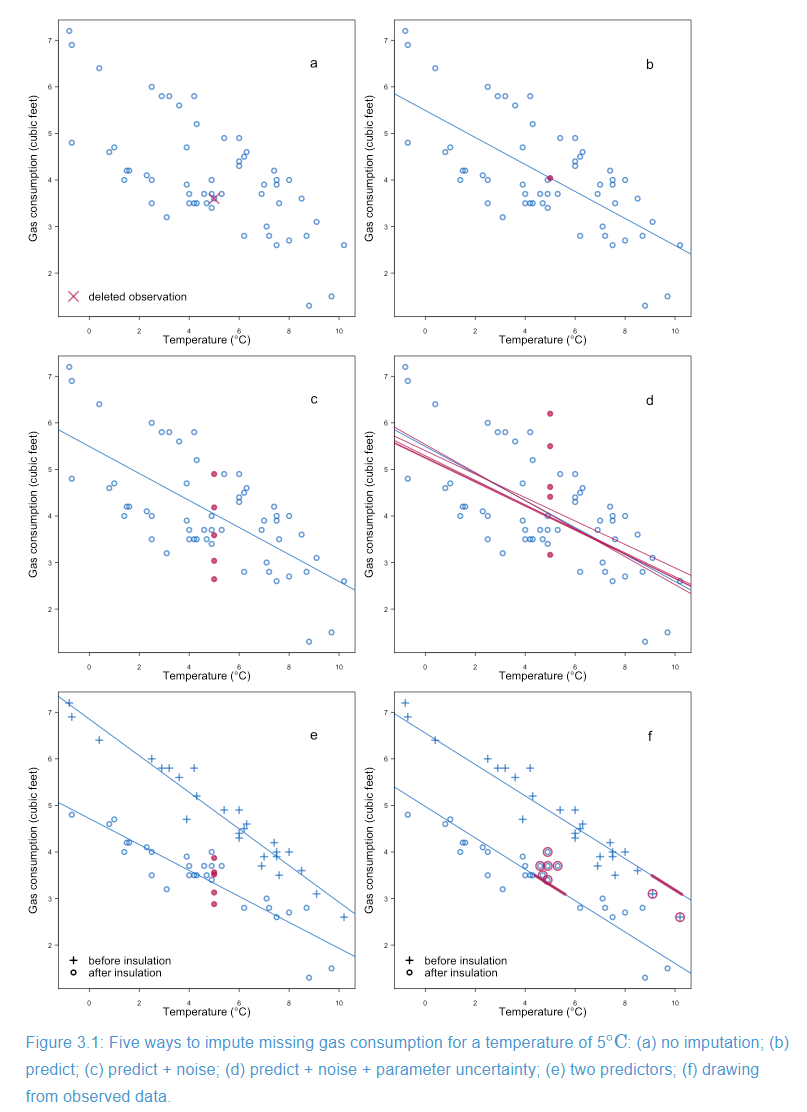
\includegraphics[width=0.55\textwidth]{assets/imputors.png}
\end{figure}

\newpage
% ─────────────────────────────────────────────────────────────────────────────

\subsection{Grundbegriffe der Kryptographie und des Hashings}

\textbf{Ziel der Kryptographie:} Sichere Übertragung von Informationen, sodass Lauscher (Eve) die Nachricht auch mit Zugang zum verschlüsselten Text nicht verstehen können. Zentral ist das \textbf{Kerckhoffs'sche Prinzip}: Die Sicherheit hängt nur vom geheimen Schlüssel ab, nicht von der Geheimhaltung des Algorithmus selbst (security through transparency, nicht obscurity).

\textbf{Symmetrische vs.\ asymmetrische Verfahren:}
\begin{itemize}[leftmargin=1.5em]
    \item \textbf{Symmetrisch:} Ein gemeinsamer Schlüssel zum Ver- und Entschlüsseln (z.\,B.\ AES, Vigenère). Effizient für große Datenmengen, aber \textbf{Schlüsselaustausch-Problem}: Wie teilt man den Schlüssel sicher mit? Lösung: Asymmetrisches Verfahren für Schlüsselaustausch, dann symmetrisch (TLS/HTTPS).
    \item \textbf{Asymmetrisch (Public Key):} Zwei komplementäre Schlüssel -- öffentlicher zum Verschlüsseln, privater zum Entschlüsseln (z.\,B.\ RSA). Ermöglicht \textbf{digitale Signaturen}: Bob verschlüsselt den Hash einer Nachricht mit seinem privaten Schlüssel; jeder kann mit Bobs öffentlichem Schlüssel prüfen, dass der Hash korrekt ist -- Authentizität ohne geteiltes Geheimnis.
\end{itemize}

\definition{\textbf{Caesar-Cipher:} Einfachster Strom-Cipher: $z \mapsto (z + k) \bmod 26$ mit Shift $k \in \{1,\ldots,25\}$. Nur 25 mögliche Schlüssel $\Rightarrow$ durch vollständige Enumeration trivial zu brechen.}

\definition{\textbf{Substitutions-Cipher:} Jeder Buchstabe wird bijektiv auf einen anderen abgebildet. $26! \approx 4 \times 10^{26}$ mögliche Zuordnungen -- klingt sicher, doch \textbf{Häufigkeitsanalyse} der Sprache (E ist häufigster Buchstabe im Deutschen/Englischen, charakteristische Bi-/Trigramme wie ``th'', ``er'', ``sch'') macht den Code knackbar. Effektive Schlüsselgröße $\ll 26!$.}

\definition{\textbf{Vigenère-Cipher:} Positionsabhängige Verschiebung $z_i \mapsto (z_i + k_{i \bmod L}) \bmod 26$ mit Schlüsselwort der Länge $L$, das periodisch wiederholt wird. Widersteht einfacher Häufigkeitsanalyse, ist aber durch den \textbf{Kasiski-Test} (Suche nach wiederkehrenden Zeichenfolgen zur Bestimmung von $L$) angreifbar.

    \textbf{One-Time Pad:} Ist der Schlüssel mindestens so lang wie die Nachricht, besteht aus unabhängig gleichverteilten Symbolen und wird \emph{nur einmal} verwendet, ist der Code \textbf{informationstheoretisch sicher} (Shannon 1949) -- ohne Kenntnis des Schlüssels ist jeder Klartext gleich plausibel. Praktisch unpraktikabel für große Datenmengen.}

\definition{\textbf{Kryptographische Hash-Funktionen:} $H: \{0,1\}^* \to \{0,1\}^n$ mit folgenden Eigenschaften:
    \begin{enumerate}[leftmargin=1.5em]
        \item \textbf{Effizienz:} Schnelle Berechnung aus Eingabe beliebiger Länge.
        \item \textbf{Kollisionsresistenz:} Praktisch unmöglich, zwei unterschiedliche Eingaben $x \neq x'$ mit $H(x) = H(x')$ zu finden.
        \item \textbf{Einwegfunktion (Preimage Resistance):} Aus Hash $h$ schwer, ein $x$ mit $H(x) = h$ zu rekonstruieren.
        \item \textbf{Avalanche-Effekt:} Kleine Änderung der Eingabe führt zu einem völlig anderen Hash (statistisch $\sim 50\,\%$ der Bits ändern sich).
    \end{enumerate}}

\textbf{Salting und Stretching:} Bei Passwort-Hashing wird ein zufälliges \textbf{Salt} (pro Benutzer) zur Eingabe hinzugefügt, bevor gehasht wird. Dadurch haben zwei Benutzer mit gleichem Passwort verschiedene Hashes -- \textbf{Rainbow Tables} (vorberechnete Hash-Tabellen) werden unwirksam. \textbf{Key Derivation Functions} wie bcrypt, scrypt oder Argon2 wenden die Hash-Funktion tausende Male iteriert an (\textbf{Stretching}): Eine einzelne Überprüfung dauert $\sim$100\,ms -- für den Benutzer unmerklich, für Brute-Force-Angreifer prohibitiv langsam.

\newpage